\chapter{Future Work}


The proposed design for video surveillance with access control using Esp Eye and HLF has been materialized. The implemented design is steered by the use case and technologies used. Considering the heterogeneous environment the solution achieved the milestones. 
In Figure~\ref{fig:relay} is a diagram which depicts how it could be realized in practice. Esp Eye has the ability to control the relay through the help of GPIOs. The Relay will then activate the electric door strike to unlock the door. 
So when a face is recognized GPIO pins will activate the Relay and it closes and then the current flows from the high power supply. 

\begin{figure}[!htb]
    \centering
    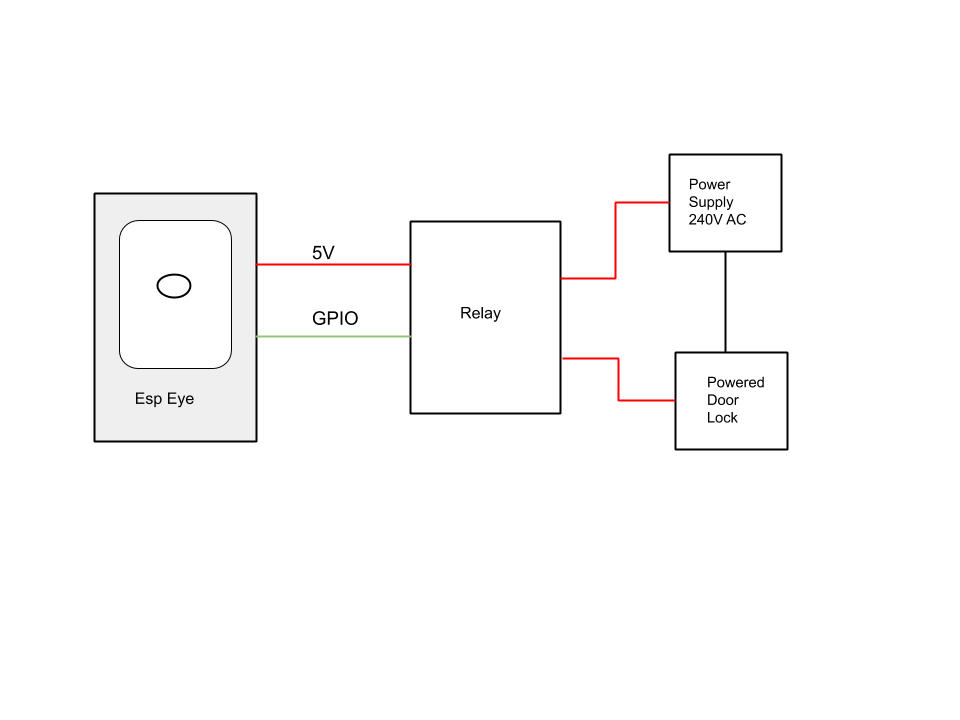
\includegraphics[width=1\textwidth]{figures/Relay.png}
    \caption{Wiring Diagram.}
    \label{fig:relay}
\end{figure}


\subsection{Limitations and Improvements}

As a first limitation is that the Esp Who platform for face detection and recognition does not provide any documentation. Nevertheless after getting familiar with it, it was possible to understand the APIs. Secondly, after a lot of research and tries we did not find any working libraries for asymmetric or symmetric encryption in Esp Eye. This is the major drawback of Esp Eye since digital integrity is important in our case. 

On the other hand Hyperledger Fabric offers signing of transactions either online or offline. In offline mode the transaction must be fabric-signed before reaching endorsing peers. Unfortunately HLF APIs for offline signing of transactions are not available for IoT devices. First of all signing of transaction requires to have Elliptic Curve Digital Signature Algorithm (ECDSA). Once this is possible in Esp Eye then the further step would be to see if HLF provides an endpoint to submit the signed transaction. 

Furthermore, Esp Eye stores the registered face IDs in the flash itself. However the idea is to fetch face IDs upon device startup from a different source which could be on the cloud. However the limitation is that the face id vector is dynamically allocated in the memory. This is due to a technical limitation in esp32 boards because the maximum statically allocated memory is 160 KB. 
There is already some contribution in this direction and the workaround is to register the face IDs from the images being fetched from an API gateway. This is implemented however the face was not recognized in the first try. 
